\section{曲面论基本定理}

为了说明 $\mathrm{I},\mathrm{II}$ 构成曲面的完全的不变量系统,需要曲面论的基本公式,也就是曲面的自然标架场的求导公式.它们在曲面的理论中扮演基本的角色,相当于曲线论中的 Frenet 公式.

Einstein 和式约定:
\begin{figure}[H]
\centering
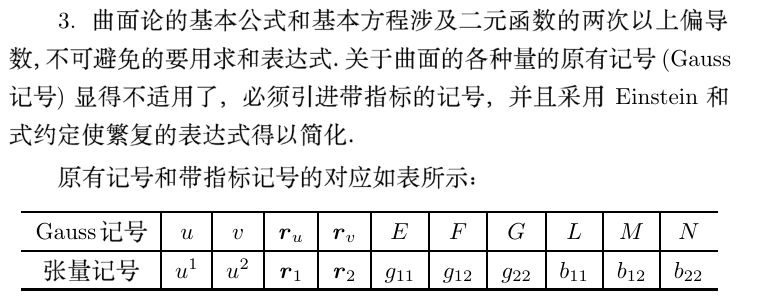
\includegraphics[width=\textwidth]{曲面论(不严谨)-2025040322.png}
% \caption{}
\label{}
\end{figure}

规定希腊字母 $\alpha,\beta,\gamma, \dots$ 作为指标的取值范围为 $\{ 1,2 \}$. 规定拉丁字母 $i,j,k,l,a,b,c,\dots$ 作为指标的取值范围为 $\{ 1,2,3 \}$.

\begin{figure}[H]
\centering
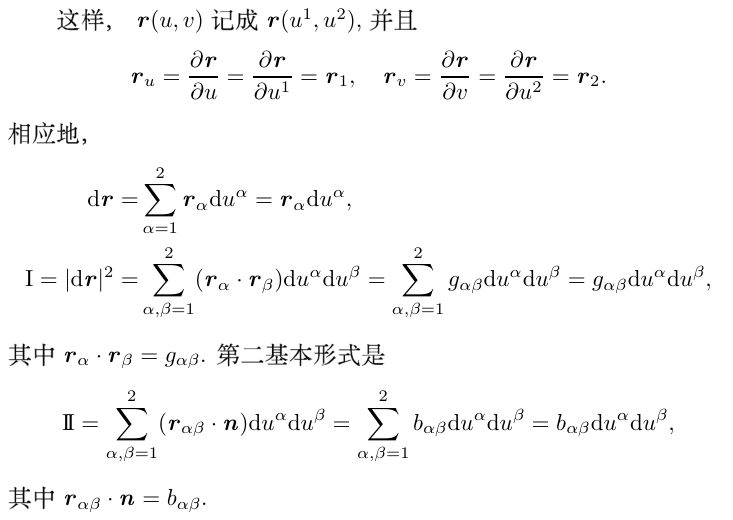
\includegraphics[width=\textwidth]{曲面论(不严谨)-2025040323.png}
% \caption{}
\label{}
\end{figure}

\subsection{Gauss 绝妙定理}

\begin{theorem}[Gauss 绝妙定理]
曲面的 Gauss 曲率是曲面在保长变换下的不变量.
\end{theorem}
事实上,由 Gauss 方程可知
\[
K=\frac{b_{11}b_{22}-(b_{12})^2}{g_{11}g_{22}-(g_{12})^2}=\frac{R_{1212}}{g_{11}g_{22}-(g_{12})^2}
\]
因此曲面的 Gauss 曲率是由它的第一基本形式完全确定的. 在 $g_{12}=F=0$ 的情形,Gauss 曲率用曲面的第一基本形式的表达式是
\[
K=-\frac{1}{\sqrt{ EG }}\left( \left( \frac{(\sqrt{ E })_{v}}{\sqrt{ G }} \right)_{v}+\left( \frac{(\sqrt{ G }_{u})}{\sqrt{ E }} \right)_{u} \right)
\]
在曲面的等温参数系下,$E=G=\lambda^{2},F=0$,则 Gauss 曲率的表达式是
\[
K=-\frac{1}{\lambda^{2}}\left( \frac{ \partial^2   }{ \partial u ^2 } +\frac{ \partial^2   }{ \partial v ^2 }  \right)\log\lambda
\]
\begin{remark}
Gauss 绝妙定理是微分几何学发展过程中的里程碑,开创了内蕴几何学的新时代,进而引发了 Riemann 几何学.
\end{remark}